\documentclass[11pt,a4paper]{article}

\usepackage[T1]{fontenc}
\usepackage[utf8]{inputenc}
\usepackage{lmodern}
\usepackage[scaled=0.95]{helvet}
\renewcommand\familydefault{\sfdefault}
\usepackage{microtype}
\usepackage[a4paper,margin=24mm,top=26mm,bottom=26mm]{geometry}
\usepackage[table]{xcolor}
\usepackage{tabularx,booktabs,array}
\usepackage{enumitem}
\usepackage{titlesec}
\usepackage{fancyhdr}
\usepackage{listings}
\usepackage{needspace}
\usepackage{tikz}
\usetikzlibrary{positioning,arrows.meta}
\usepackage[hidelinks]{hyperref}

\definecolor{ink}{HTML}{1F2933}
\definecolor{muted}{HTML}{616E7C}
\definecolor{rule}{HTML}{CBD2D9}
\definecolor{accent}{HTML}{2563EB}
\definecolor{good}{HTML}{15803D}
\definecolor{warn}{HTML}{B45309}
\definecolor{bad}{HTML}{B91C1C}

\color{ink}
\setlength{\parindent}{0pt}
\setlength{\parskip}{6pt}
\renewcommand{\arraystretch}{1.35}
\setlist{itemsep=1pt,topsep=3pt,leftmargin=16pt}

\titleformat{\section}{\Large\bfseries\color{ink}}{}{0pt}{}[\vspace{2pt}{\color{rule}\titlerule[0.6pt]}]
\titlespacing*{\section}{0pt}{14pt}{6pt}

\pagestyle{fancy}
\fancyhf{}
\fancyhead[L]{\small\color{muted}DoT Front-end}
\fancyhead[R]{\small\color{muted}Design and progress}
\fancyfoot[C]{\small\color{muted}\thepage}
\renewcommand{\headrulewidth}{0pt}

\lstset{basicstyle=\ttfamily\small,backgroundcolor=\color{rule!35},frame=none,
        xleftmargin=8pt,framexleftmargin=8pt,aboveskip=6pt,belowskip=6pt,columns=flexible,
        keepspaces=true}

\newcommand{\done}{\textcolor{good}{\textbf{Done}}}
\newcommand{\todo}{\textcolor{muted}{Remaining}}

\begin{document}

\thispagestyle{empty}
{\Huge\bfseries DoT Front-end}\par
\vspace{4pt}
{\Large\color{muted} Design and progress}\par
\vspace{6pt}
{\small\color{muted} Owner: Dhruv \quad$\cdot$\quad 20 October 2026}\par
\vspace{14pt}

The front-end is the resolver's front door. It accepts encrypted DNS queries from clients over
DNS-over-TLS (TCP port 853), checks each one, passes valid queries to the middleware, and sends
back the encrypted answers. It also decides which clients and queries get rejected, and how.

We are implementing all of the features below. \textbf{5 of 11 are complete}; the rest are in
progress.

\section{How a query flows through the front-end}

\begin{center}
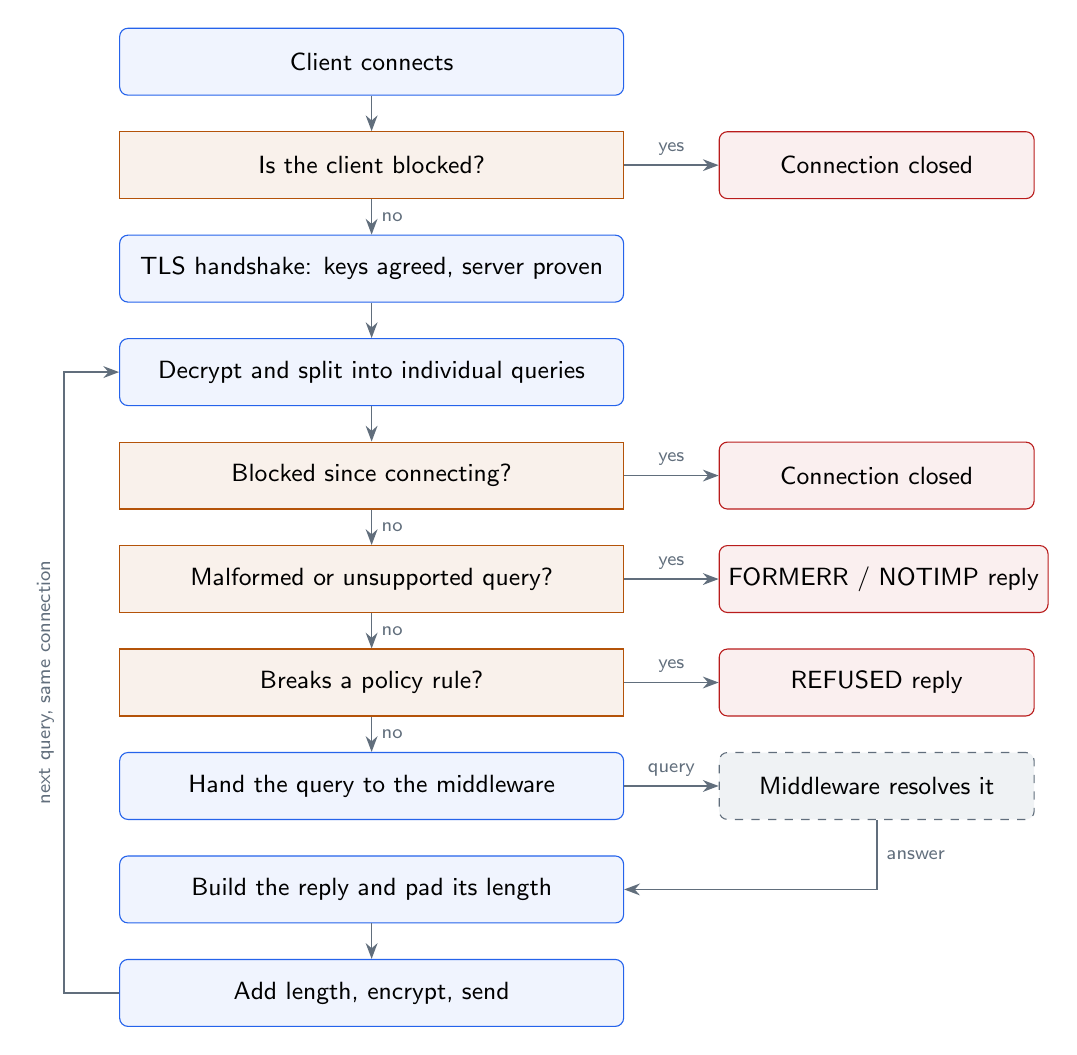
\begin{tikzpicture}[
  node distance=4.5mm and 12mm,
  base/.style={rectangle, minimum width=64mm, minimum height=8.5mm, align=center, font=\small},
  flow/.style={base, rounded corners=3pt, draw=accent, fill=accent!7},
  check/.style={base, draw=warn, fill=warn!8},
  reject/.style={rectangle, rounded corners=3pt, draw=bad, fill=bad!7, minimum width=40mm,
                 minimum height=8.5mm, align=center, font=\small},
  ext/.style={rectangle, rounded corners=3pt, draw=muted, dashed, fill=rule!30, minimum width=40mm,
              minimum height=8.5mm, align=center, font=\small},
  arr/.style={-{Stealth[length=2mm]}, semithick, draw=muted},
  lbl/.style={font=\scriptsize, text=muted}
]
\node[flow]                   (connect)   {Client connects};
\node[check, below=of connect]   (blocked1)  {Is the client blocked?};
\node[flow,  below=of blocked1]  (tls)       {TLS handshake: keys agreed, server proven};
\node[flow,  below=of tls]       (decrypt)   {Decrypt and split into individual queries};
\node[check, below=of decrypt]   (blocked2)  {Blocked since connecting?};
\node[check, below=of blocked2]  (malformed) {Malformed or unsupported query?};
\node[check, below=of malformed] (policy)    {Breaks a policy rule?};
\node[flow,  below=of policy]    (submit)    {Hand the query to the middleware};
\node[flow,  below=of submit]    (build)     {Build the reply and pad its length};
\node[flow,  below=of build]     (send)      {Add length, encrypt, send};

\node[reject, right=of blocked1]  (close1)  {Connection closed};
\node[reject, right=of blocked2]  (close2)  {Connection closed};
\node[reject, right=of malformed] (formerr) {FORMERR / NOTIMP reply};
\node[reject, right=of policy]    (refused) {REFUSED reply};
\node[ext,    right=of submit]    (mw)      {Middleware resolves it};

\draw[arr] (connect) -- (blocked1);
\draw[arr] (blocked1) -- node[lbl, right] {no} (tls);
\draw[arr] (tls) -- (decrypt);
\draw[arr] (decrypt) -- (blocked2);
\draw[arr] (blocked2) -- node[lbl, right] {no} (malformed);
\draw[arr] (malformed) -- node[lbl, right] {no} (policy);
\draw[arr] (policy) -- node[lbl, right] {no} (submit);
\draw[arr] (build) -- (send);

\draw[arr] (blocked1) -- node[lbl, above] {yes} (close1);
\draw[arr] (blocked2) -- node[lbl, above] {yes} (close2);
\draw[arr] (malformed) -- node[lbl, above] {yes} (formerr);
\draw[arr] (policy) -- node[lbl, above] {yes} (refused);

\draw[arr] (submit) -- node[lbl, above] {query} (mw);
\draw[arr] (mw.south) |- node[lbl, pos=0.25, right] {answer} (build.east);

\draw[arr] (send.west) -- ++(-7mm,0) |- node[lbl, pos=0.25, rotate=90, above] {next query, same connection} (decrypt.west);
\end{tikzpicture}
\end{center}

A connection stays open after a reply, so one client can send many queries without repeating
the TLS handshake.

\clearpage
\section{Features}

\begin{tabularx}{\linewidth}{@{}>{\bfseries\raggedright\arraybackslash}p{37mm}X>{\raggedright\arraybackslash}p{19mm}@{}}
\toprule
\normalfont\textbf{Feature} & \textbf{What it does} & \textbf{Status} \\
\midrule
Query parsing and validation & Turns raw bytes into a checked query; rejects anything malformed or
  hostile without ever reading outside the message & \done \\
Name normalization & Treats \texttt{WWW.Example.COM} and \texttt{www.example.com.} as the same name,
  and rejects invalid names & \done \\
Reply building & Turns the middleware's answer into a correct DNS reply, always producing a valid
  message (falls back to SERVFAIL if needed) & \done \\
Length padding & Pads replies to a fixed block size so encrypted traffic doesn't reveal which site
  was looked up by its size & \done \\
Message framing & Splits the decrypted byte stream into individual queries, and prefixes each reply
  with its length & \done \\
\midrule
TLS encryption & Encrypts every connection with OpenSSL; sets up keys securely and proves the
  server's identity & \todo \\
Abuse blocking & Drops clients the middleware has flagged as abusive, before spending any work on
  them & \todo \\
Policy rejections & Answers REFUSED for queries that break a rule, such as a blocked domain & \todo \\
Connection handling & Serves many clients at once, several queries per connection, with timeouts
  and connection limits & \todo \\
Configuration & Listen address, certificate and key paths, limits, blocked-domain list & \todo \\
Runnable server & A server binary that can be tested end to end with \texttt{dig +tls} & \todo \\
\bottomrule
\end{tabularx}

\needspace{14\baselineskip}
\section{How the front-end rejects queries}

\begin{tabularx}{\linewidth}{@{}>{\raggedright\arraybackslash}p{58mm}>{\raggedright\arraybackslash}p{38mm}X@{}}
\toprule
\textbf{Situation} & \textbf{Response} & \textbf{Why} \\
\midrule
Client flagged as abusive by the middleware & Connection closed, no reply & No work or bandwidth
  spent on attackers \\
Message too broken to read its ID, or not a query at all & Connection closed, no reply & There is
  nothing valid to reply to \\
Malformed query & FORMERR & Tells a buggy client what's wrong \\
Query kind we don't support & NOTIMP & A clear answer instead of silence \\
Query breaks a policy rule & REFUSED & A clear answer for legitimate clients \\
Middleware is overloaded & SERVFAIL & The client can retry later \\
\bottomrule
\end{tabularx}

\needspace{16\baselineskip}
\section{What the response codes mean}

Every DNS reply carries a response code. FORMERR, NOTIMP and REFUSED say the problem is with the
query, so sending it again won't help; SERVFAIL says the problem is on the resolver's side, so
retrying later can succeed.

{\renewcommand{\arraystretch}{1.25}
\begin{tabularx}{\linewidth}{@{}>{\raggedright\arraybackslash}p{33mm}>{\raggedright\arraybackslash}X>{\raggedright\arraybackslash}p{17mm}@{}}
\toprule
\textbf{Code} & \textbf{What it means in this resolver} & \textbf{Retry?} \\
\midrule
\textbf{FORMERR}\newline{\small\color{muted}Format error \textperiodcentered{} code 1} &
  \textbf{The query is broken.} It was readable enough to reply to, but breaks DNS rules: wrong
  section counts, a damaged or invalid name, a bad EDNS record, or extra bytes at the end & No \\
\textbf{NOTIMP}\newline{\small\color{muted}Not implemented \textperiodcentered{} code 4} &
  \textbf{Valid, but unsupported.} It asks for an operation other than a standard query, a class
  other than Internet (e.g.\ CHAOS), or a record type we don't handle yet (e.g.\ HTTPS) & No \\
\textbf{REFUSED}\newline{\small\color{muted}Refused \textperiodcentered{} code 5} &
  \textbf{Understood, but not allowed.} The query is valid and supported, but a policy rule
  forbids answering it, such as a blocked domain & No \\
\textbf{SERVFAIL}\newline{\small\color{muted}Server failure \textperiodcentered{} code 2} &
  \textbf{No answer could be produced.} The query was fine, but the middleware was overloaded,
  the upstream servers failed, or the answer couldn't be turned into a valid reply &
  \textcolor{good}{Yes}, later \\
\bottomrule
\end{tabularx}}

\needspace{14\baselineskip}
\section{How the encryption works}

\begin{itemize}
  \item \textbf{The session key is never sent.} Client and server each compute it from a key
        exchange (ECDHE), so someone watching the network can't obtain it.
  \item \textbf{The server proves its identity} by signing the handshake with its private key.
        The key never leaves the server, and the signature stops anyone impersonating it.
  \item \textbf{Forward secrecy.} A stolen private key would let an attacker impersonate the
        server in future, but not decrypt traffic recorded earlier.
  \item \textbf{Length padding} covers the one thing TLS doesn't hide: message sizes.
  \item \textbf{Key file protection.} The private key file is readable only by the server, and
        key files are kept out of git.
\end{itemize}

\section{What the front-end needs from the middleware}

The middleware is built separately by a teammate. The front-end relies on two things from it:

\begin{itemize}
  \item \textbf{A way to submit a query.} The middleware either accepts it and answers later,
        rejects the client, or reports that it's overloaded.
  \item \textbf{A blocklist the front-end can check.} It answers ``is this client blocked right
        now?''
\end{itemize}

\section{Running the tests}

\begin{lstlisting}
make CXX=g++ test    # build and run all tests
make CXX=g++ asan    # same tests with memory-error detection
\end{lstlisting}

\end{document}
